\begin{name}
	{\tenchude}
	{\tendethi}
	{.}
	{.}
\end{name}
\setcounter{ex}{0}\setcounter{bt}{0}
\Opensolutionfile{ans}[ans/ans-2-GHK1-4-NguyenKhuyen-TPHCM-20]
\begin{ex}%[GHKI-Kiểm tra định kỳ lớp 12, Nguyễn Khuyến, HCM]%[Đỗ Viết Lân, Ex1-2020]%[2D1Y2-1]
	Hàm số $y=x^3+3x^2+2$ có điểm cực đại là
	\choice
	{$0$}
	{$6$}
	{$2$}
	{\True $-2$}
	\loigiai{
		Tập xác định: $\mathscr{D}=\mathbb{R}$.\\
		Ta có $y'=3x^2+6x$, $y'=0\Leftrightarrow \hoac{&x=0 \Rightarrow y=2\\&x=-2 \Rightarrow y=6.}$\\
		Bảng biến thiên
		\begin{center}
			
\begin{tikzpicture}
			\tkzTabInit
			[lgt=1.2,espcl=2.5] % tùy chọn
			{$x$/0.8, $f’(x)$/0.8, $f(x)$/1.8} % cột đầu tiên
			{$-\infty$, $-2$, $0$, $+\infty$} % hàng 1 cột 2
			\tkzTabLine{,+,0,-,0,+,} % hàng 2 cột 2
			\tkzTabVar{-/ $-\infty$, +/ $6$, -/ $2$,  +/ $+\infty$} % hàng 3 cột 2
			\end{tikzpicture}
		\end{center}
		Vậy hàm số có điểm cực đại là $x_{\text{CĐ}}=-2$.
	}
\end{ex}

\begin{ex}%[GHKI-Kiểm tra định kỳ lớp 12, Nguyễn Khuyến, HCM]%[Đỗ Viết Lân, Ex1-2020]%[2D1Y5-6]
	Phương trình tiếp tuyến của đồ thị hàm số $y=x^3+3x^2+2$ tại điểm có hoành độ bằng $-2$ là
	\choice
	{$y=0$}
	{\True $y=6$}
	{$y=x$}
	{$y=x+2$}
	\loigiai{
		Ta có $y'=3x^2+6x\Rightarrow y'(-2) = 0$.\\
		Phương trình tiếp tuyến của đồ thị hàm số $y=x^3+3x^2+2$ tại điểm có hoành độ bằng $-2$ là
		$$y=y'(-2)(x+2)+y(-2)\Leftrightarrow y=6.$$
	}
\end{ex}

\begin{ex}%[GHKI-Kiểm tra định kỳ lớp 12, Nguyễn Khuyến, HCM]%[Đỗ Viết Lân, Ex1-2020]%[2D1Y1-2]
	Cho hàm số $y=f(x)$ có bảng biến thiên như hình vẽ. Hàm số $y=f(x)$ nghịch biến trên khoảng nào sau đây?
	\begin{center}
		
\begin{tikzpicture}
		\tkzTabInit
		[lgt=1.2,espcl=2.5] % tùy chọn
		{$x$/0.6, $f’(x)$/0.6, $f(x)$/2} % cột đầu tiên
		{$-\infty$, $-1$, $0$, $1$, $+\infty$} % hàng 1 cột 2
		\tkzTabLine{,-,0,+,0,-,0,+,} % hàng 2 cột 2
		\tkzTabVar{+/ $+\infty$, -/ $0$, +/ $\dfrac{5}{2}$, -/ $0$ , +/ $+\infty$} % hàng 3 cột 2
		\end{tikzpicture}
	\end{center}
	\choice
	{\True $(-\infty;-2)$}
	{$(-\infty;0)$}
	{$(-1;0)$}
	{$(0;+\infty)$}
	\loigiai{
		Hàm số $y=f(x)$ nghịch biến trên khoảng $(-\infty;-2)$.
	}
\end{ex}

\begin{ex}%[GHKI-Kiểm tra định kỳ lớp 12, Nguyễn Khuyến, HCM]%[Đỗ Viết Lân, Ex1-2020]%[2D1Y4-1]
	Cho hàm số $y=\dfrac{x^2+1}{x^2-4}$. Số đường tiệm cận của đồ thị hàm số là
	\choice
	{$1$}
	{$4$}
	{$2$}
	{\True $3$}
	\loigiai{
		\begin{itemize}
			\item $\lim\limits_{x\to \pm\infty} y=1$ nên đồ thị hàm số có tiệm cận ngang $y=1$.
			\item $\lim\limits_{x\to 2^+} y=+\infty, \lim\limits_{x\to 2^-} y=-\infty  $ nên đồ thị hàm số có tiệm cận đứng $x=2$.
			\item $\lim\limits_{x\to (-2)^+} y=-\infty, \lim\limits_{x\to (-2)^-} y=+\infty  $ nên đồ thị hàm số có tiệm cận đứng $x=-2$.
		\end{itemize}
	}
\end{ex}

\begin{ex}%[GHKI-Kiểm tra định kỳ lớp 12, Nguyễn Khuyến, HCM]%[Đỗ Viết Lân, Ex1-2020]%[2H1B3-2]
	Tính thể tích của khối chóp tứ giác đều có cạnh đáy bằng $a$ và cạnh bên bằng $b$.
	\choice
	{\True $\dfrac {a^{2}\sqrt {4b^{2}-2a^{2}}}{6}$}
	{$\dfrac {a^{2}\sqrt {4b^{2}-a^{2}}}{6}$}
	{$\dfrac {a^{2}\sqrt {4b^{2}+2a^{2}}}{6}$}
	{$\dfrac {a^{2}\sqrt {4b^{2}+a^{2}}}{6}$}
	\loigiai{
		\immini{
			Gọi $O$ là giao điểm của $AC$ và $BD$.\\
			Ta có $SO\perp(ABCD) \Rightarrow SO$ là đường cao.\\
			Thể tích khối chóp $S.ABCD$ 
			$$V_{S.ABCD}=\dfrac{1}{3}\cdot SO\cdot S_{ABCD}.$$
			Trong đó 
			\begin{itemize}
				\item $S_{ABCD}=a^2$.
				\item $SC=b,OC=\dfrac{a\sqrt{2}}{2} \\ \Rightarrow SO=\sqrt{SC^2-OC^2}=\dfrac{\sqrt{4b^2-2a^2}}{2}$.
			\end{itemize}
			Vậy $V_{S.ABCD}=\dfrac {a^{2}\sqrt {4b^{2}-2a^{2}}}{6}$.
		}{
			\begin{tikzpicture}[scale=0.7, font=\footnotesize, line join=round, line cap=round, >=stealth]
			\tkzDefPoints{0/0/A, -2.5/-2/B, 3/-2/C}
			\coordinate (D) at ($(A)+(C)-(B)$);
			\coordinate (O) at ($(A)!.5!(C)$);
			\coordinate (S) at ($(O)+(0,4)$);
			\tkzDrawSegments[dashed](S,A A,B A,D A,C B,D S,O)
			\tkzDrawSegments(S,B S,C S,D B,C C,D)
			\tkzDrawPoints[fill=black](S,A,B,C,D,O)
			%\tkzLabelPoints(A,B,C,D,O,S,M)
			\tkzLabelPoints[left=0.1](A)
			\tkzLabelPoints[below left](B)
			\tkzLabelPoints[below right](C,D)
			\tkzLabelPoints[above](S)
			\tkzLabelPoints[below](O)
			\end{tikzpicture}
		}
	}
\end{ex}

\begin{ex}%[GHKI-Kiểm tra định kỳ lớp 12, Nguyễn Khuyến, HCM]%[Đỗ Viết Lân, Ex1-2020]%[2D1B5-1]
	Đường cong ở hình vẽ là đồ thị của hàm số nào trong bốn hàm số dưới đây?
	\begin{center}
		\begin{tikzpicture}[scale=1, line join=round, line cap=round,font=\footnotesize,>=stealth,x=1cm,y=1cm]
		\draw[->] (-1.5,0)--(0,0) node[below left]{$O$}--(3.5,0) node [below] {$x$};
		\draw[->] (0,-2.5)--(0,2.5) node [left] {$y$};
		\foreach \x in {-1,1,2,3}
		\draw (\x,0.05)--(\x,-0.05) node [below] {\x};
		\foreach \y in {-2,-1,1,2}
		\draw (0.05,\y)--(-0.05,\y) node [left] {\y};
		\draw[black,domain=-1:3, samples=100]plot(\x,{(\x)^3-3*(\x)^2+2});
		\end{tikzpicture}
	\end{center}
	\choice
	{$y=-x^{3}+3x^{2}+2$}
	{$y=-x^{3}+3x^{2}+1$}
	{\True $y=x^{3}-3x^{2}+2$}
	{$y=x^{3}+3x^{2}+2$}
	\loigiai{
		Đồ thị hàm số đi qua điểm $(0;2)$ và $(1;0)$ nên chỉ có đồ thị hàm số $y=x^{3}-3x^{2}+2$ thỏa mãn trong $4$ hàm số đã cho trong đáp án.
	}
\end{ex}

\begin{ex}%[GHKI-Kiểm tra định kỳ lớp 12, Nguyễn Khuyến, HCM]%[Đỗ Viết Lân, Ex1-2020]%[1H3B5-3]
	Tính chiều cao của hình chóp tứ giác đều có cạnh đáy bằng $a$ và cạnh bên bằng $b$.
	\choice
	{$\dfrac{\sqrt{4b^2+2a^2}}{2}$}
	{\True $\dfrac{\sqrt{4b^2-2a^2}}{2}$}
	{$\dfrac{\sqrt{4b^2-a^2}}{2}$}
	{$\dfrac{\sqrt{4b^2+a^2}}{2}$}
	\loigiai{
		Giả sử $S.ABCD$ là hình chóp đều và $O=AC \cap BD$. Khi đó $ABCD$ là hình vuông và $SO\perp (ABCD)$.
		\immini{
			$SC=b,OC=\dfrac{a\sqrt{2}}{2} \\ \Rightarrow SO=\sqrt{SC^2-OC^2}=\dfrac{\sqrt{4b^2-2a^2}}{2}$.\\
			Vậy chiều cao của khối chóp là $SO=\dfrac{\sqrt{4b^2-2a^2}}{2}$.
		}{
			\begin{tikzpicture}[scale=0.7, font=\footnotesize, line join=round, line cap=round, >=stealth]
			\tkzDefPoints{0/0/A, -2.5/-2/B, 3/-2/C}
			\coordinate (D) at ($(A)+(C)-(B)$);
			\coordinate (O) at ($(A)!.5!(C)$);
			\coordinate (S) at ($(O)+(0,4)$);
			\tkzDrawSegments[dashed](S,A A,B A,D A,C B,D S,O)
			\tkzDrawSegments(S,B S,C S,D B,C C,D)
			\tkzDrawPoints[fill=black](S,A,B,C,D,O)
			%\tkzLabelPoints(A,B,C,D,O,S,M)
			\tkzLabelPoints[left=0.1](A)
			\tkzLabelPoints[below left](B)
			\tkzLabelPoints[below right](C,D)
			\tkzLabelPoints[above](S)
			\tkzLabelPoints[below](O)
			\end{tikzpicture}
		}
	}
\end{ex}

\begin{ex}%[GHKI-Kiểm tra định kỳ lớp 12, Nguyễn Khuyến, HCM]%[Đỗ Viết Lân, Ex1-2020]%[1H3B5-4]
	Cho hình lập phương $ABCD.A'B'C'D'$. Góc giữa hai đường thẳng $AC$ và $DA'$ bằng
	\choice
	{$120^\circ$}
	{$45^\circ$}
	{\True $60^\circ$}
	{$90^\circ$}
	\loigiai{
		\immini{
			Ta có $CB'\parallel DA'$ nên $(AC,DA')=(AC,CB')$.\\
			Xét tam giác $AB'C$ có $AB'=B'C=CA$ nên tam giác $AB'C$ đều.\\
			Vậy góc giữa hai đường thẳng $AC$ và $DA'$ là
			$$(AC,DA')=(AC,CB')=60^{\circ}.$$
		}{
			\begin{tikzpicture}[scale=0.8, font=\footnotesize, line join=round, line cap=round, >=stealth]
			\tkzDefPoints{3/2/x, 4/0/y, 0/4/z, 0/0/A}
			\coordinate (B) at ($(A)+(x)$);
			\coordinate (C) at ($(B)+(y)$);
			\coordinate (D) at ($(C)-(x)$);
			\coordinate (A') at ($(A)+(z)$);
			\coordinate (B') at ($(B)+(z)$);
			\coordinate (D') at ($(D)+(z)$);
			\coordinate (C') at ($(C)+(z)$);
			\tkzDrawSegments[dashed](A,B B,C B,B' A,C C,B' B',A)
			\tkzDrawSegments(A,D D,C A,A' D,D' C,C' A',B' B',C' C',D' D',A' D,A')
			%\tkzLabelPoints(A,B,C,D,A',B',C',D',O)
			\tkzDrawPoints[fill=black](A,B,C,D,A',B',C',D')
			\tkzLabelPoints[above](A',B',C',D')
			\tkzLabelPoints[below](A,B,C,D)
			\end{tikzpicture}}
	}
\end{ex}

\begin{ex}%[GHKI-Kiểm tra định kỳ lớp 12, Nguyễn Khuyến, HCM]%[Đỗ Viết Lân, Ex1-2020]%[2D1Y2-2]
	Cho hàm số $y=f(x)$ liên tục trên $\mathbb{R}$ và có bảng xét dấu của đạo hàm như hình vẽ. Hàm số đã cho có bao nhiêu điểm cực trị?
	\begin{center}
		
\begin{tikzpicture}
		\tkzTabInit
		[lgt=1.2,espcl=2.5] % tùy chọn
		{$x$/0.8, $f’(x)$/0.8} % cột đầu tiên
		{$-\infty$, $-1$, $0$, $2$, $4$, $+\infty$} % hàng 1 cột 2
		\tkzTabLine{,+,0,-,d,+,0,-,0,+,}
		\end{tikzpicture}
	\end{center}
	\choice
	{\True $4$}
	{$2$}
	{$1$}
	{$3$}
	\loigiai{
		Ta có hàm số $y=f(x)$ liên tục trên $\mathbb{R}$ và $f'(x)$ đổi dấu $4$ lần nên hàm số có $4$ điểm cực trị.
	}
\end{ex}

\begin{ex}%[GHKI-Kiểm tra định kỳ lớp 12, Nguyễn Khuyến, HCM]%[Đỗ Viết Lân, Ex1-2020]%[1H3B5-3]
	Cho hình chóp tứ giác đều $S.ABCD$ có cạnh đáy bằng $a$ và chiều cao bằng $h$. Gọi $O$ là tâm của đáy $ABCD$. Tính khoảng cách từ $O$ đến mặt phẳng $(SAB)$.
	\choice
	{$\dfrac{ah}{\sqrt{2a^2+4h^2}}$}
	{\True $\dfrac{ah}{\sqrt{a^2+4h^2}}$}
	{$\dfrac{ah}{\sqrt{a^2+h^2}}$}
	{$\dfrac{ah}{2\sqrt{a^2+h^2}}$}
	\loigiai{
		$S.ABCD$ là hình chóp đều nên $SO\perp(ABCD)$.
		\immini{
			Gọi $I$ là trung điểm của $AB$.\\
			Ta có $\heva{&AB \perp OI\\&AB \perp SO} \Rightarrow AB \perp (SOI)$.\\
			Kẻ $OH \perp SI$ tại $H$.\\
			Ta có $\heva{&OH \perp SI\\&OH \perp AB} \Rightarrow OH \perp (SAB)$.\\
			Suy ra $\mathrm{d}(O,(SAB))=OH$.\\
			Xét tam giác $SOI$ vuông tại $O$, đường cao $OH$ có\\
			$\dfrac{1}{OH^2}=\dfrac{1}{SO^2}+\dfrac{1}{OI^2}\Leftrightarrow \dfrac{1}{OH^2}=\dfrac{1}{h^2}+\dfrac{1}{\left (\dfrac{a}{2}\right )^2}$\\
			$\Rightarrow OH=\dfrac{ah}{\sqrt{a^2+4h^2}}$.\\
			Vậy $\mathrm{d}(O,(SAB))=\dfrac{ah}{\sqrt{a^2+4h^2}}$.
		}{
			\begin{tikzpicture}[scale=0.8, font=\footnotesize, line join=round, line cap=round, >=stealth]
			\tkzDefPoints{0/0/D, -2.5/-2/C, 3/-2/B}
			\coordinate (A) at ($(D)+(B)-(C)$);
			\coordinate (O) at ($(A)!.5!(C)$);
			\coordinate (S) at ($(O)+(0,5)$);
			\coordinate (I) at ($(A)!.5!(B)$);
			\coordinate (H) at ($(S)!.65!(I)$);
			\tkzDrawSegments[dashed](C,D S,D A,D A,C B,D S,O O,I O,H)
			\tkzDrawSegments(S,A A,B S,B S,C B,C S,I)
			\tkzDrawPoints[fill=black](S,A,B,C,D,O,I,O,H)
			%\tkzLabelPoints(A,B,C,D,O,S,M)
			\tkzLabelPoints[left=0.1](D)
			\tkzLabelPoints[below left](C)
			\tkzLabelPoints[below right](A,B,I)
			\tkzLabelPoints[right](H)
			\tkzLabelPoints[above](S)
			\tkzLabelPoints[below](O)
			\tkzMarkRightAngles(O,H,I O,I,B)
			\end{tikzpicture}}
	}
\end{ex}

\begin{ex}%[GHKI-Kiểm tra định kỳ lớp 12, Nguyễn Khuyến, HCM]%[Đỗ Viết Lân, Ex1-2020]%[2D1B1-1]
	Cho hàm số $y=f(x)$ có đạo hàm $f'(x) = (x+1)^2(x-1)^3(2-x)$. Hàm số $y=f(x)$ đồng biến trên khoảng nào dưới đây?
	\choice
	{$(2;+\infty)$}
	{$(-\infty;1)$}
	{\True $(1;2)$}
	{$(-1;1)$}
	\loigiai{
		Theo đề bài ta có bảng biến thiên sau
		\begin{center}
			
\begin{tikzpicture}
			\tkzTabInit
			[lgt=1.2,espcl=2.5] % tùy chọn
			{$x$/0.8, $f’(x)$/0.8, $f(x)$/2} % cột đầu tiên
			{$-\infty$, $-1$, $1$, $2$, $+\infty$} % hàng 1 cột 2
			\tkzTabLine{,-,0,-,0,+,0,-,} % hàng 2 cột 2
			\tkzTabVar{+/ $+\infty$, R/ , -/ , +/  , -/ $-\infty$} % hàng 3 cột 2
			\end{tikzpicture}
		\end{center}
	}
\end{ex}

\begin{ex}%[GHKI-Kiểm tra định kỳ lớp 12, Nguyễn Khuyến, HCM]%[Đỗ Viết Lân, Ex1-2020]%[2H1Y3-2]
	Thể tích của khối lăng trụ tam giác đều $ABC.A'B'C'$ có $AB=a$, $AA'=b$ là
	\choice
	{\True $\dfrac{a^2b\sqrt{3}}{4}$}
	{$\dfrac{a^2b\sqrt{3}}{12}$}
	{$\dfrac{a^2b\sqrt{3}}{2}$}
	{$\dfrac{a^2b\sqrt{3}}{6}$}
	\loigiai{
		\immini{
			Thể tích của khối lăng trụ tam giác đều $ABC.A'B'C'$ là
			$$V_{ABC.A'B'C'}=S_{ABC}\cdot AA'=\dfrac{a^2\sqrt{3}}{4}\cdot b =\dfrac{a^2b\sqrt{3}}{4}.$$
		}{
			\begin{tikzpicture}[scale=0.7, font=\footnotesize, line join=round, line cap=round, >=stealth]
			\tkzDefPoints{0/0/A, 2/-2/B, 5/0/C, 0/5/z}
			\coordinate (A') at ($(A)+(z)$);
			\coordinate (B') at ($(B)+(z)$);
			\coordinate (C') at ($(C)+(z)$);
			\tkzDrawPolygon(A',B',C')
			\tkzDrawSegments(A,A' A,B B,C B,B' C,C')
			\tkzDrawSegments[dashed](A,C)
			\tkzLabelPoints[below right](B, C, B',C')
			\tkzLabelPoints[left](A, A')
			\tkzLabelSegment[left](A,A'){$b$}
			\tkzLabelSegment[left](A,B){$a$}
			\tkzDrawPoints(A,B,C,A',B',C')
			\end{tikzpicture}}
	}
\end{ex}

\begin{ex}%[GHKI-Kiểm tra định kỳ lớp 12, Nguyễn Khuyến, HCM]%[Đỗ Viết Lân, Ex1-2020]%[2H1B3-2]
	Cho lăng trụ tam giác đều $ABC.A'B'C'$ có $AB=a$, $AA'=b$ và điểm $M$ là điểm thuộc cạnh $AA'$. Thể tích khối tứ diện $BCB'M$ bằng
	\choice
	{$\dfrac{a^2b\sqrt{3}}{4}$}
	{$\dfrac{a^2b\sqrt{3}}{6}$}
	{$\dfrac{a^2b\sqrt{3}}{8}$}
	{\True $\dfrac{a^2b\sqrt{3}}{12}$}
	\loigiai{
		\immini{Do $AA'\parallel (BCC'B')\Rightarrow \mathrm{d}(A,(BCC'B'))=\mathrm{d}(M,(BCC'B'))\\ \Rightarrow V_{M.BCC'B'}=V_{A.BCC'B'}$.\\
			Vì $V_{A.A'B'C'}=\dfrac{1}{3}V_{ABC.A'B'C'}$ nên $V_{A.BCC'B'}=\dfrac{2}{3}V_{ABC.A'B'C'}$.\\
			Lúc này ta có
			\begin{align*}
			V_{M.BCB'}&=\dfrac{1}{2}V_{M.BCC'B'}\\
			&=\dfrac{1}{2}V_{A.BCC'B'}\\
			&=\dfrac{1}{2}\cdot \dfrac{2}{3}V_{ABC.A'B'C'}\\
			&=\dfrac{1}{3}V_{ABC.A'B'C'}\\
			&=\dfrac{1}{3}\cdot \dfrac{a^2b\sqrt{3}}{4}=\dfrac{a^2b\sqrt{3}}{12}.
			\end{align*}}{
			\begin{tikzpicture}[scale=0.6, font=\footnotesize, line join=round, line cap=round, >=stealth]
			\tkzDefPoints{0/0/A, 2/-2/B, 5/0/C, 0/5/z}
			\coordinate (A') at ($(A)+(z)$);
			\coordinate (B') at ($(B)+(z)$);
			\coordinate (C') at ($(C)+(z)$);
			\coordinate (M) at ($(A)!0.3!(A')$);
			\tkzDrawPolygon(A',B',C')
			\tkzDrawSegments(A,A' A,B B,C B,B' C,C' B',C B',M B,M)
			\tkzDrawSegments[dashed](A,C M,C)
			\tkzLabelPoints[below right](B, C,C')
			\tkzLabelPoints[above](B')
			\tkzLabelPoints[left](A, A',M)
			\tkzLabelSegment[left](A,A'){$b$}
			\tkzLabelSegment[left](A,B){$a$}
			\tkzDrawPoints[fill=black](A,B,C,A',B',C',M)
			\end{tikzpicture}
		}
	}
\end{ex}

\begin{ex}%[GHKI-Kiểm tra định kỳ lớp 12, Nguyễn Khuyến, HCM]%[Đỗ Viết Lân, Ex1-2020]%[2D1K5-3]
	Cho hàm số $y=f(x)$ có đồ thị trên đoạn $[-2;4]$ như hình vẽ. Khẳng định đúng là
	\begin{center}
		\begin{tikzpicture}[scale=1, line join=round, line cap=round,font=\footnotesize,>=stealth,x=1cm,y=1cm]
		\draw[->] (-2.5,0)--(0,0) node[below left]{$O$}--(4.5,0) node [below] {$x$};
		\draw[->] (0,-3.5)--(0,2.5) node [left] {$y$};
		\foreach \x in {-2,-1,1,2,3,4}
		\draw (\x,0.05)--(\x,-0.05) node [below] {\x};
		\foreach \y in {-2,-1,1,2,-3}
		\draw (0.05,\y)--(-0.05,\y) node [left] {\y};
		\draw[black,domain=-2:-1, samples=100]plot(\x,{-2*(\x)-5});
		\draw[black,domain=-1:2, samples=100]plot(\x,{5*(\x)/3-4/3});
		\draw[black,domain=2:4, samples=100]plot(\x,{-(\x)/2+3});
		\draw[dashed] (-2,0)--(-2,-1)--(0,-1) (-1,0)--(-1,-3)--(0,-3) (2,0)--(2,2)--(0,2) (4,0)--(4,1)--(0,1);
		\end{tikzpicture}
	\end{center}
	\choice
	{Điểm cực đại của đồ thị hàm số là $2$}
	{Phương trình $f(x)=0$ có $3$ nghiệm $x\in[-2;4]$}
	{\True $f'\left(-\dfrac{3}{2}\right)f(0)>0$}
	{$\max\limits_{[-2;4]} f(x)=4$}
	\loigiai{
		Theo đồ thị ta thấy $f(0) < 0$ và $f'\left(-\dfrac{3}{2}\right)<0$ (do hàm số nghịch biến trên khoảng $(-2;-1)$) nên $f'\left(-\dfrac{3}{2}\right)f(0)>0$.
	}
\end{ex}

\begin{ex}%[GHKI-Kiểm tra định kỳ lớp 12, Nguyễn Khuyến, HCM]%[Đỗ Viết Lân, Ex1-2020]%[1H3B5-4]
	Cho hình lập phương $ABCD.A'B'C'D'$ có cạnh bằng $a$ và $I$ là trung điểm $CD'$. Tính khoảng cách giữa hai đường thẳng $BI$ và $B'C'$.
	\choice
	{\True $\dfrac{a\sqrt{2}}{2}$}
	{$a\sqrt{2}$}
	{$\dfrac{a\sqrt{3}}{2}$}
	{$\dfrac{a}{2}$}
	\loigiai{
		\begin{center}
			\begin{tikzpicture}[scale=0.8, font=\footnotesize, line join=round, line cap=round, >=stealth]
			\tkzDefPoints{2/1/x, 4/0/y, 0/4/z, 0/0/A}
			\coordinate (B) at ($(A)+(x)$);
			\coordinate (C) at ($(B)+(y)$);
			\coordinate (D) at ($(C)-(x)$);
			\coordinate (A') at ($(A)+(z)$);
			\coordinate (B') at ($(B)+(z)$);
			\coordinate (D') at ($(D)+(z)$);
			\coordinate (C') at ($(C)+(z)$);
			\coordinate (I) at ($(C)!.5!(D')$);
			\tkzDrawSegments[dashed](A,B B,C B,B' B,I B,A')
			\tkzDrawSegments(A,D D,C A,A' D,D' C,C' A',B' B',C' C',D' D',A' C,D')
			%\tkzLabelPoints(A,B,C,D,A',B',C',D',O)
			\tkzDrawPoints[fill=black](A,B,C,D,A',B',C',D',I)
			\tkzLabelPoints[above](A',B',C',D')
			\tkzLabelPoints[below](A,B,C,D,I)
			\end{tikzpicture}
		\end{center}
		Ta có $BI \subset (BCD'A'), B'C' \parallel(BCD'A')$.\\
		Suy ra $\mathrm{d}(BI,B'C')=\mathrm{d}(B'C',(BCD'A'))=\mathrm{d}(C',(BCD'A'))=C'I=\dfrac{a\sqrt{2}}{2}$.
	}
\end{ex}

\begin{ex}%[GHKI-Kiểm tra định kỳ lớp 12, Nguyễn Khuyến, HCM]%[Đỗ Viết Lân, Ex1-2020]%[1H3B5-4]
	Cho hình chóp tứ giác đều $S.ABCD$ có cạnh đáy bằng $a$ và chiều cao $h$. Tính khoảng cách giữa hai đường thẳng $AC$ và $SB$.
	\choice
	{$\dfrac{ah}{\sqrt{2a^2+4h^2}}$}
	{$\dfrac{ah}{\sqrt{a^2+4h^2}}$}
	{\True $\dfrac{ah}{\sqrt{a^2+2h^2}}$}
	{$\dfrac{ah}{2\sqrt{a^2+2h^2}}$}
	\loigiai{
		\immini{
			Ta có $AC\perp BD$ và $AC\perp SO$ nên $AC\perp (SBD)$.\\
			Từ $O$ kẻ $OH\perp SB$ tại $H$. Khi đó $OH\perp AC$.\\
			Suy ra $\rm{d}(AC;SB)=OH$.\\
			Lại có $\dfrac{1}{OH^2}=\dfrac{1}{SO^2}+\dfrac{1}{OB^2}\Rightarrow OH = \dfrac{ah}{\sqrt{a^2+2h^2}}$
		}
		{\begin{tikzpicture}[scale=0.7, font=\footnotesize, line join=round, line cap=round, >=stealth]
			\tkzDefPoints{0/0/A, -2.5/-2/B, 3/-2/C}
			\coordinate (D) at ($(A)+(C)-(B)$);
			\coordinate (O) at ($(A)!.5!(C)$);
			\coordinate (S) at ($(O)+(0,4)$);
			\coordinate (H) at ($(S)!.6!(B)$);
			\tkzDrawSegments[dashed](S,A A,B A,D A,C B,D S,O O,H)
			\tkzDrawSegments(S,B S,C S,D B,C C,D)
			\tkzDrawPoints[fill=black](S,A,B,C,D,O,H)
			%\tkzLabelPoints(A,B,C,D,O,S,M)
			\tkzLabelPoints[left=0.1](A)
			\tkzLabelPoints[below left](B)
			\tkzLabelPoints[left](H)
			\tkzLabelPoints[below right](C,D)
			\tkzLabelPoints[above](S)
			\tkzLabelPoints[below](O)
			\end{tikzpicture}}
	}
\end{ex}

\begin{ex}%[GHKI-Kiểm tra định kỳ lớp 12, Nguyễn Khuyến, HCM]%[Đỗ Viết Lân, Ex1-2020]%[2D1B2-1]
	Cho hàm số $y=f(x)$ có đạo hàm $f'(x) = x^2(x+3)^2(x^2-9)(x-1)^3$. Số điểm cực trị của hàm số là
	\choice
	{$4$}
	{$1$}
	{$2$}
	{\True $3$}
	\loigiai{
		Ta có bảng biến thiên
		\begin{center}
			
\begin{tikzpicture}
			\tkzTabInit
			[lgt=1.2,espcl=2.5] % tùy chọn
			{$x$/0.8, $f’(x)$/0.8, $f(x)$/2} % cột đầu tiên
			{$-\infty$, $-3$, $0$,$1$,$3$, $+\infty$} % hàng 1 cột 2
			\tkzTabLine{,-,0,+,0,+,0,-,0,+,}
			\tkzTabVar{+/ , -/ , R/,+/ , -/, +/} % hàng 3 cột 2
			\end{tikzpicture}
		\end{center}
		Suy ra hàm số có ba điểm cực trị.
	}
\end{ex}

\begin{ex}%[GHKI-Kiểm tra định kỳ lớp 12, Nguyễn Khuyến, HCM]%[Đỗ Viết Lân, Ex1-2020]%[1D5B2-1]
	Trong giờ học toán cô giáo ghi 1 bài tập toán trên bảng và gọi $2$ học sinh lên giải. Câu hỏi ``Cho hàm số $y=f(x)=x^2+4x$. Tính đạo hàm của hàm số $y=f(3x)$.''\\
	Học sinh thứ nhất giải: $f'(x)=2x+4\Rightarrow f'(3x) = 6x+4$.\\
	Học sinh thứ hai giải: $f(3x)=(3x)^2+4(3x) \Rightarrow f'(3x) = 18x+12$.\\
	Lời giải của học sinh nào đúng?
	\choice
	{Hai học sinh đều sai}
	{\True Học sinh thứ hai}
	{Học sinh thứ nhất}
	{Hai học sinh đều đúng}
	\loigiai{
		Theo công thức đạo hàm, chỉ có học sinh thứ hai làm đúng.
	}
\end{ex}

\begin{ex}%[GHKI-Kiểm tra định kỳ lớp 12, Nguyễn Khuyến, HCM]%[Đỗ Viết Lân, Ex1-2020]%[2D1B4-1]
	Cho hàm số $y=f(x)$ xác định trên $\mathbb{R}\setminus\{-1\}$, liên tục trên mỗi khoảng xác định và có bảng biến thiên như hình vẽ và có đồ thị $(C)$. Khẳng định nào sau đây \textbf{sai}?
	\begin{center}
		
\begin{tikzpicture}
		\tkzTabInit
		[lgt=1.2,espcl=2.5] % tùy chọn
		{$x$/0.8, $f’(x)$/0.8, $f(x)$/2} % cột đầu tiên
		{$-\infty$, $-1$, $1$, $+\infty$} % hàng 1 cột 2
		\tkzTabLine{,+,d,+,0,-,}
		\tkzTabVar{-/ $1$, +D-/ $3$ /$-\infty$ , +/ $2$, -/ $-1$} % hàng 3 cột 2
		\end{tikzpicture}
	\end{center}
	\choice
	{\True Đồ thị $(C)$ không có tiệm cận đứng}
	{$\max\limits_{(-1;+\infty)}f(x)=2$}
	{Hàm số có điểm cực đại $x=1$}
	{Hàm số không có đạo hàm tại điểm $x=-1$}
	\loigiai{
		Dựa vào bảng biến thiên đồ thị $(C)$ có tiệm cận đứng $x=-1$.
	}
\end{ex}

\begin{ex}%[GHKI-Kiểm tra định kỳ lớp 12, Nguyễn Khuyến, HCM]%[Đỗ Viết Lân, Ex1-2020]%[2D1B1-1]
	Hàm số $y=27x+\dfrac{4}{x^2}$ đồng biến trên khoảng nào?
	\choice
	{$(-\infty;28)$}
	{\True $\left(\dfrac{2}{3};+\infty\right)$}
	{$(-27;+\infty)$}
	{$(0;25)$}
	\loigiai{
		$D = \mathbb{R}\setminus\{0\}$.\\
		Ta có $y'=27-\dfrac{8}{x^3}$.\\
		Do đó $y' > 0 \Leftrightarrow x>\dfrac{2}{3}$ hoặc $x<0$. Khoảng đồng biến cần tìm là $\left(\dfrac{2}{3};+\infty\right)$
	}
\end{ex}
\begin{ex}%[Giữa HK1-Nguyễn Khuyến-HCM, 2019-20120]%[Sang Nguyen, 12EX1]%[2D1K3-1]
	\immini
	{Cho hàm số $y=f(x)$ liên tục trên $\mathbb{R}$ và có đồ thị hàm số $y=f'(x)$ như hình vẽ. Hàm số $y=f(x)$ đạt giá trị nhỏ nhất trên đoạn $\left[0;\dfrac{7}{2}\right]$ tại điểm nào dưới đây?
		\choice 
		{$x_0=0$}
		{$x_0=1$}
		{$x_0=\dfrac{7}{2}$}
		{\True $x_0=3$}
	}
	{ \begin{tikzpicture}[line join = round, line cap = round,>=stealth,font=\footnotesize,scale=0.7]
		\def\xt{-1} \def\xp{4.3} \def\yd{-3} \def\yt{3.5}
		\draw[->] (\xt,0)--(\xp,0) node[below]{$x$};
		\draw[->] (0,\yd)--(0,\yt) node[left]{$y$};
		\fill (0,0) circle (1.5pt) node[below left]{$O$};
		\begin{scope}
		\clip (\xt+0.1,\yd+0.1) rectangle (\xp-0.1,\yt-0.1);
		\draw[samples=100,domain=\xt:\xp,smooth] plot (\x, {1/1.5*(\x-1)^2*(\x-3)});
		\end{scope}
		\draw[dashed] (3.5,0)node[below]{$\dfrac{7}{2}$}--(3.5,2.083);
		\node at (1,0)[above]{$1$};
		\node at (3,0)[above left]{$3$};
		\end{tikzpicture}
	} 
	\loigiai{
		Dự vào đồ thị của hàm số $y=f'(x)$, ta có bảng biến thiên sau:
		\begin{center}
			
\begin{tikzpicture}
			\tkzTabInit[nocadre=false,lgt=1.2,espcl=2.5,deltacl=0.6]{$x$/.6 ,$f'(x)$/.6,$f(x)$/2}
			{$0$ ,$1$, $3$ , $\tfrac{7}{2}$}
			\tkzTabLine{ , - , $0$ ,-,$0$, + , }
			\tkzTabVar{+/ ,R, -/$f(3)$ , +/}
			\end{tikzpicture}
		\end{center}
		Dựa vào bảng biến thiên trên, ta có giá trị nhỏ nhất trên đoạn $\left[0;\dfrac{7}{2}\right]$ là $f(3)$.} 
\end{ex} 
\begin{ex}%[Giữa HK1-Nguyễn Khuyến-HCM, 2019-20120]%[Sang Nguyen, 12EX1]%[2D1B1-3]
	Hàm số $y=-x^3+3x^2+3mx$ nghịch biến trên $\mathbb{R}$ khi
	\choice 
	{$m\ge-1$}
	{\True $m\le-1$}
	{$m\ge-2$}
	{$m\le 3$} 
	\loigiai{
		Ta có $y'=-3x^2+6x+3m$.\\
		Hàm số nghịch biến trên $\mathbb{R}\Leftrightarrow y'\le 0,\,\forall x\in\mathbb{R}\Leftrightarrow\Delta '=9+9m\le 0\Leftrightarrow m\le-1$.} 
\end{ex} 
\begin{ex}%[Giữa HK1-Nguyễn Khuyến-HCM, 2019-20120]%[Sang Nguyen, 12EX1]%[2H1B2-3]
	Số mặt phẳng đối xứng của hình lập phương là
	\choice 
	{$6$}
	{$8$}
	{$7$}
	{\True $9$} 
	\loigiai{
		\begin{center}
			\begin{tikzpicture}[line join = round, line cap = round,>=stealth,font=\footnotesize,scale=0.7]
			\tkzDefPoints{0/0/A,-2/-1/B,1/-1/C}
			\coordinate (D) at ($(A)+(C)-(B)$);
			\coordinate (A') at ($(A)+(0,2.5)$);
			\tkzDefPointsBy[translation=from A to A'](B,C,D){B'}{C'}{D'}
			\tkzDrawPolygon[draw = white, fill= gray, opacity=.4](A,C,C',A')
			\tkzDrawPolygon(A',B',B,C,D,D')
			\tkzDrawSegments(B',C' C',D' C,C')
			\tkzDrawSegments[dashed](A,B A,D A,A')
			\end{tikzpicture} $\quad$ $\quad$
			\begin{tikzpicture}[line join = round, line cap = round,>=stealth,font=\footnotesize,scale=0.7]
			\tkzDefPoints{0/0/A,-2/-1/B,1/-1/C}
			\coordinate (D) at ($(A)+(C)-(B)$);
			\coordinate (A') at ($(A)+(0,2.5)$);
			\tkzDefPointsBy[translation=from A to A'](B,C,D){B'}{C'}{D'}
			\tkzDrawPolygon[draw = white, fill= gray, opacity=.4](B,D,D',B')
			\tkzDrawPolygon(A',B',B,C,D,D')
			\tkzDrawSegments(B',C' C',D' C,C')
			\tkzDrawSegments[dashed](A,B A,D A,A')
			\end{tikzpicture} $\quad$ $\quad$
			\begin{tikzpicture}[line join = round, line cap = round,>=stealth,font=\footnotesize,scale=0.7]
			\tkzDefPoints{0/0/A,-2/-1/B,1/-1/C}
			\coordinate (D) at ($(A)+(C)-(B)$);
			\coordinate (A') at ($(A)+(0,2.5)$);
			\tkzDefPointsBy[translation=from A to A'](B,C,D){B'}{C'}{D'}
			\coordinate (M) at ($(C)!1/2!(B)$);
			\coordinate (N) at ($(C')!1/2!(B')$);
			\coordinate (P) at ($(A)!1/2!(D)$);
			\coordinate (Q) at ($(A')!1/2!(D')$);
			\tkzDrawPolygon[draw = white, fill= gray, opacity=.4](M,N,Q,P)
			\tkzDrawPolygon(A',B',B,C,D,D')
			\tkzDrawSegments(B',C' C',D' C,C')
			\tkzDrawSegments[dashed](A,B A,D A,A')
			\end{tikzpicture}\\
			\begin{tikzpicture}[line join = round, line cap = round,>=stealth,font=\footnotesize,scale=0.7]
			\tkzDefPoints{0/0/A,-2/-1/B,1/-1/C}
			\coordinate (D) at ($(A)+(C)-(B)$);
			\coordinate (A') at ($(A)+(0,2.5)$);
			\tkzDefPointsBy[translation=from A to A'](B,C,D){B'}{C'}{D'}
			\coordinate (M) at ($(A)!1/2!(B)$);
			\coordinate (N) at ($(A')!1/2!(B')$);
			\coordinate (P) at ($(C)!1/2!(D)$);
			\coordinate (Q) at ($(C')!1/2!(D')$);
			\tkzDrawPolygon[draw = white, fill= gray, opacity=.4](M,N,Q,P)
			\tkzDrawPolygon(A',B',B,C,D,D')
			\tkzDrawSegments(B',C' C',D' C,C')
			\tkzDrawSegments[dashed](A,B A,D A,A')
			\end{tikzpicture} $\quad$ $\quad$
			\begin{tikzpicture}[line join = round, line cap = round,>=stealth,font=\footnotesize,scale=0.7]
			\tkzDefPoints{0/0/A,-2/-1/B,1/-1/C}
			\coordinate (D) at ($(A)+(C)-(B)$);
			\coordinate (A') at ($(A)+(0,2.5)$);
			\tkzDefPointsBy[translation=from A to A'](B,C,D){B'}{C'}{D'}
			\coordinate (M) at ($(A)!1/2!(A')$);
			\coordinate (N) at ($(B)!1/2!(B')$);
			\coordinate (P) at ($(C)!1/2!(C')$);
			\coordinate (Q) at ($(D)!1/2!(D')$);
			\tkzDrawPolygon[draw = white, fill= gray, opacity=.4](M,N,P,Q)
			\tkzDrawPolygon(A',B',B,C,D,D')
			\tkzDrawSegments(B',C' C',D' C,C')
			\tkzDrawSegments[dashed](A,B A,D A,A')
			\end{tikzpicture} $\quad$ $\quad$
			\begin{tikzpicture}[line join = round, line cap = round,>=stealth,font=\footnotesize,scale=0.7]
			\tkzDefPoints{0/0/A,-2/-1/B,1/-1/C}
			\coordinate (D) at ($(A)+(C)-(B)$);
			\coordinate (A') at ($(A)+(0,2.5)$);
			\tkzDefPointsBy[translation=from A to A'](B,C,D){B'}{C'}{D'}
			\tkzDrawPolygon[draw = white, fill= gray, opacity=.4](A',D',C,B)
			\tkzDrawPolygon(A',B',B,C,D,D')
			\tkzDrawSegments(B',C' C',D' C,C')
			\tkzDrawSegments[dashed](A,B A,D A,A')
			\end{tikzpicture} \\
			\begin{tikzpicture}[line join = round, line cap = round,>=stealth,font=\footnotesize,scale=0.7]
			\tkzDefPoints{0/0/A,-2/-1/B,1/-1/C}
			\coordinate (D) at ($(A)+(C)-(B)$);
			\coordinate (A') at ($(A)+(0,2.5)$);
			\tkzDefPointsBy[translation=from A to A'](B,C,D){B'}{C'}{D'}
			\tkzDrawPolygon[draw = white, fill= gray, opacity=.4](A,D,C',B')
			\tkzDrawPolygon(A',B',B,C,D,D')
			\tkzDrawSegments(B',C' C',D' C,C')
			\tkzDrawSegments[dashed](A,B A,D A,A')
			\end{tikzpicture} $\quad$ $\quad$
			\begin{tikzpicture}[line join = round, line cap = round,>=stealth,font=\footnotesize,scale=0.7]
			\tkzDefPoints{0/0/A,-2/-1/B,1/-1/C}
			\coordinate (D) at ($(A)+(C)-(B)$);
			\coordinate (A') at ($(A)+(0,2.5)$);
			\tkzDefPointsBy[translation=from A to A'](B,C,D){B'}{C'}{D'}
			\tkzDrawPolygon[draw = white, fill= gray, opacity=.4](A',B',C,D)
			\tkzDrawPolygon(A',B',B,C,D,D')
			\tkzDrawSegments(B',C' C',D' C,C')
			\tkzDrawSegments[dashed](A,B A,D A,A')
			\end{tikzpicture} $\quad$ $\quad$
			\begin{tikzpicture}[line join = round, line cap = round,>=stealth,font=\footnotesize,scale=0.7]
			\tkzDefPoints{0/0/A,-2/-1/B,1/-1/C}
			\coordinate (D) at ($(A)+(C)-(B)$);
			\coordinate (A') at ($(A)+(0,2.5)$);
			\tkzDefPointsBy[translation=from A to A'](B,C,D){B'}{C'}{D'}
			\tkzDrawPolygon[draw = white, fill= gray, opacity=.4](A,B,C',D')
			\tkzDrawPolygon(A',B',B,C,D,D')
			\tkzDrawSegments(B',C' C',D' C,C')
			\tkzDrawSegments[dashed](A,B A,D A,A')
			\end{tikzpicture} 
		\end{center}
	} 
\end{ex} 
\begin{ex}%[Giữa HK1-Nguyễn Khuyến-HCM, 2019-20120]%[Sang Nguyen, 12EX1]%[1D1B3-1]
	Số nghiệm của phương trình $\cos 2x-\cos x+1=0$ trên $\left[0;\dfrac{\pi}{2}\right]$ là
	\choice 
	{\True $2$}
	{$3$}
	{$1$}
	{$0$} 
	\loigiai{
		Ta có $\cos 2x-\cos x+1=0\Leftrightarrow 2{\cos}^2x-\cos x=0$ 
		$\Leftrightarrow\hoac{&\cos x=0\\&\cos x=\dfrac{1}{2}}\Leftrightarrow\hoac{&x=\dfrac{\pi}{2}+k\pi\\&x=\pm\dfrac{\pi}{3}+k2\pi}(k\in\mathbb{Z})$.\\
		Suy ra số nghiệm của phương trình trong $\left[0;\dfrac{\pi}{2}\right]$ là $2$.} 
\end{ex} 
\begin{ex}%[Giữa HK1-Nguyễn Khuyến-HCM, 2019-20120]%[Sang Nguyen, 12EX1]%[2D1B4-1] 
	Số đường tiệm cận ngang của đồ thị hàm số $y=\dfrac{x-2\sqrt{x^2-x}}{2x-3}$ là
	\choice 
	{$1$}
	{$3$}
	{\True $2$}
	{$4$} 
	\loigiai{
		Hàm số xác định khi và chỉ khi $\heva {&x^2-x\ge 0\\&2x-3\ne 0}\Leftrightarrow\heva {&x\le 0\vee x\ge 1\\&x\ne\dfrac{3}{2}.}$\\
		Tập xác định $\mathscr{D}=\left(-\infty ;0\right]\cup\left[1;\dfrac{3}{2}\right)\cup \left(\dfrac{3}{2};+\infty \right)$.\\
		Ta có:
		$\lim\limits_{x\to+\infty}y=\lim\limits_{x\to+\infty}\dfrac{x-2\sqrt{x^2-x}}{2x-3}=\lim\limits_{x\to+\infty}\dfrac{x\left( 1-2\sqrt{1-\dfrac{1}{x}}\right) }{x\left(2-\dfrac{3}{x}\right)}=\lim\limits_{x\to+\infty}\dfrac{1-2\sqrt{1-\dfrac{1}{x}}}{2-\dfrac{3}{x}}=-\dfrac{1}{2}$.\\
		$\lim\limits_{x\to-\infty}y=\lim\limits_{x\to-\infty}\dfrac{x-2\sqrt{x^2-x}}{2x-3}=\lim\limits_{x\to-\infty}\dfrac{x\left( 1+2\sqrt{1-\dfrac{1}{x}}\right) }{x\left( 2-\dfrac{3}{x}\right) }=\lim\limits_{x\to-\infty}\dfrac{1+2\sqrt{1-\dfrac{1}{x}}}{2-\dfrac{3}{x}}=\dfrac{3}{2}$.\\
		Đường thẳng $y=-\dfrac{1}{2};\,y=\dfrac{3}{2}$ là các tiệm cận ngang của đồ thị hàm số.} 
\end{ex} 
\begin{ex}%[Giữa HK1-Nguyễn Khuyến-HCM, 2019-20120]%[Sang Nguyen, 12EX1]%[2D1B1-1]
	Cho hàm số $y=x^3-3x^2$ có giá trị lớn nhất, giá trị nhỏ nhất trên đoạn $\left[0;4\right]$ lần lượt là $M, m.$ Khẳng định đúng là
	\choice 
	{$M+m=16$}
	{\True $M+m=12$}
	{$M-m=16$}
	{$M-m=17$} 
	\loigiai{
		Hàm số xác định và liên tục trên đoạn $\left[0;4\right]$.\\
		Ta có: $y'=3x^2-6x=0\Leftrightarrow\hoac{&x=0\\&x=2.}$\\
		Ta có $y(0)=0$, $y(4)=16,y(2)=-4$. Suy ra $M=16;m=-4$, $M+m=12$.} 
\end{ex} 
\begin{ex}%[Giữa HK1-Nguyễn Khuyến-HCM, 2019-20120]%[Sang Nguyen, 12EX1]%[2D1B5-3] 
	Cho phương trình $x^3-3x^2=m$ $(*)$. Khẳng định nào sau đây \textbf{sai}?
	\choice 
	{$(*)$ có nghiệm $x\in\left[0;4\right]$ khi và chỉ khi $m\in\left[-4;16\right]$} 
	{$(*)$ có $3$ nghiệm phân biệt khi và chỉ khi $m\in (-4;0)$} 
	{$(*)$ có $3$ nghiệm phân biệt $x_1, x_2, x_3$ thỏa $x_1<0<x_2<x_3$ khi và chỉ khi $m\in (-4;0)$} 
	{\True $(*)$ có nghiệm $x\in (4;+\infty )$ khi và chỉ khi $m\in (-\infty ;16)$} 
	\loigiai{
		Xét hàm số $y=f(x)=x^3-3x^2.$ Ta có $f'(x)=3x^2-6x=0\Leftrightarrow\hoac{&x=0\\&x=2.}$\\
		Bảng biến thiên
		\begin{center}
			
\begin{tikzpicture}[>=stealth]
			\tkzTabInit[nocadre=false,lgt=1.2,espcl=2.5,deltacl=0.6]{$x$/.6 ,$y'$/.6,$y$/2}
			{$-\infty$ , $0$ , $2$ , $+\infty$}
			\tkzTabLine{ , + , $0$ , - , $0$ , + , }
			\tkzTabVar{-/$-\infty$ , +/$0$ , -/$-4$ , +/$+\infty$}
			\end{tikzpicture}
		\end{center}
		Dựa vào bảng biến thiên, ta có có hàm số $f(x)$ đồng biến trên khoảng $(2;+\infty )$, nên với $x>4$ thì $f(x)>f(4)=16$. Suy ra với $m<16$ thì phương trình $(*)$ không có nghiệm $x>4$.} 
\end{ex} 
\begin{ex}%[Giữa HK1-Nguyễn Khuyến-HCM, 2019-20120]%[Sang Nguyen, 12EX1]%[2D1K3-1] 
	Giá trị nhỏ nhất của hàm số $y=|\sqrt{4-x^2}-9|$ trên đoạn $\left[-2;2\right]$ bằng 
	\choice 
	{$0$}
	{$6$}
	{\True $7$}
	{$9$} 
	\loigiai{
		Tập xác định: $\mathscr{D}=\left[-2;2\right]$. Xét $g(x)=\sqrt{4-x^2}-9$.\\ 
		$g'(x)=0\Leftrightarrow\dfrac{-x}{\sqrt{4-x^2}}=0\Leftrightarrow x=0$.\\ 
		Ta có $g(-2)=-9,g(0)=-7,g(2)=-9$. Suy ra $\min\limits_{\left[-2;2\right]}y=7$.} 
\end{ex} 
\begin{ex}%[Giữa HK1-Nguyễn Khuyến-HCM, 2019-20120]%[Sang Nguyen, 12EX1]%[2D1B2-1] 
	Cho hàm số $y=x^4-2x^2$ có $3$ điểm cực trị là $x_1$, $x_2$, $x_3$. Khẳng định nào sau đây đúng? 
	\choice 
	{$x_1^2+x_2^2+x_3^2=16$}
	{\True $x_1+x_2+x_3=0$}
	{$x_1x_2x_3=1$}
	{$x_1+x_2+x_3=2$} 
	\loigiai{
		Tập xác định: $\mathscr{D}=\mathbb{R}$.\\
		$y'=0\Leftrightarrow 4x^3-4x=0\Leftrightarrow\hoac{&x=0\\&x=1\\&x=-1}\Rightarrow x_1+x_2+x_3=0$.} 
\end{ex} 
\begin{ex}%[Giữa HK1-Nguyễn Khuyến-HCM, 2019-20120]%[Sang Nguyen, 12EX1]%[2D1Y3-1] 
	Giá trị lớn nhất, giá trị nhỏ nhất của hàm số $y=\sqrt{4-x}$ trên đoạn $\left[-5;3\right]$ lần lượt là $M, m$. Khẳng định đúng là 
	\choice 
	{$M+m=-4$}
	{$M-m=6$}
	{\True $M+m=4$}
	{$M-m=17$} 
	\loigiai{
		Tập xác định: $\mathscr{D}=\left(-\infty ;4\right]$.\\ 
		Ta có: $y'=\dfrac{-1}{2\sqrt{4-x}}<0,\,\forall x\in \left(-\infty ;4\right)$.\\ 
		$\Rightarrow\heva {&M=\max\limits_{\left[-5;3\right]}y=y(-5)=3\\&m=\min\limits_{\left[-5;3\right]}y=y(3)=1}$ 
		$\Rightarrow M+m=4$.} 
\end{ex} 
\begin{ex}%[Giữa HK1-Nguyễn Khuyến-HCM, 2019-20120]%[Sang Nguyen, 12EX1]%[1H3K5-3] 
	Cho lăng trụ tam giác đều $ABC.A_1B_1C_1$ có $AB=a$, $AA_1=h$. Tính khoảng cách từ $A$ đến mặt phẳng $(BCA_1)$.
	\choice 
	{$\dfrac{\sqrt{3a^2+4h^2}}{4}$}
	{$\dfrac{2\sqrt{3a^2+4h^2}}{3}$}
	{$\dfrac{ah\sqrt{3}}{2\sqrt{3a^2+4h^2}}$}
	{\True $\dfrac{ah\sqrt{3}}{\sqrt{3a^2+4h^2}}$} 
	\loigiai{
		\immini{
			Gọi $H$	là trung điểm cạnh $BC$, $K$ là hình chiếu vuông gốc của $A$ lên $AH$. Ta có $AH\perp BC$ và $BC\perp AA_1$ nên $BC\perp (AA_1H)$, suy ra $BC\perp AK$ mà $AK\perp A_1H$ nên $AK\perp (A_1BC)$. Do đó $\mathrm{d}(A, (A_1BC))=AK$.\\
			Xét tam giác $A_1AH$ vuông tại $A$, ta có
			\begin{eqnarray*}
				AK&=&\dfrac{AA_1\cdot AH }{\sqrt{AA_1^2+AH^2}}=\dfrac{h\cdot \dfrac{a\sqrt{3}}{2}}{\sqrt{h^2+\left(\dfrac{a\sqrt{3}}{2}\right)^2}}\\&=&\dfrac{\dfrac{ah\sqrt{3}}{2}}{\sqrt{\dfrac{4h^2+3a^2}{4}}}=\dfrac{ah\sqrt{3}}{\sqrt{3a^2+4h^2}}.
			\end{eqnarray*}
		}
		{
			\begin{tikzpicture}[line join = round, line cap = round,>=stealth,font=\footnotesize,scale=1]
			\coordinate[label=left:$A$] (A) at (0,0);
			\coordinate[label=below left:$B$] (B) at (1,-1);
			\coordinate[label=right:$C$] (C) at (4,0);
			\coordinate[label=left:$A_1$] (A_1) at ($(A)+(90:3)$);
			\coordinate[label=below left:$B_1$] (B_1) at ($(B)-(A)+(A_1)$);
			\coordinate[label=right:$C_1$] (C_1) at ($(C)-(A)+(A_1)$);
			\coordinate[label=below:$H$] (H) at ($(B)!0.5!(C)$);
			\coordinate (K) at ($(A_1)!0.7!(H)$);
			\draw (A_1)--(A)--(B)--(C)--(C_1)--(A_1)--(B_1)--(C_1) (B)--(B_1) (A_1)--(B);
			\draw[dashed] (A)--(C)--(A_1) (K)--(A)--(H)--(A_1);
			\fill (A)circle(1.5pt) (B)circle(1.5pt) (C)circle(1.5pt) (A_1)circle(1.5pt) (B_1)circle(1.5pt) (C_1)circle(1.5pt) (H) circle(1.5pt) (K) circle(1.5pt);
			\draw[] ($(K)!5pt!(A)$)--($(K)!5pt!(A)+(K)!5pt!(H)-(K)$)--($(K)!5pt!(H)$)--(K)--cycle;
			\fill[black] (K)node[shift={(30:6pt)}]{$K$} circle (1.5pt);	 
			\end{tikzpicture}
		}
		
	} 
\end{ex} 
\begin{ex}%[Giữa HK1-Nguyễn Khuyến-HCM, 2019-20120]%[Sang Nguyen, 12EX1]%[2D1B2-1] 
	Cho hàm số $y=x^3-3x$ có hai điểm cực trị là $x_1, x_2.$ Giá trị biểu thức $P=x_1^2+x_2^2+3x_1x_2$ là 
	\choice 
	{$1$}
	{$2$}
	{\True $-1$}
	{$-2$} 
	\loigiai{
		Tập xác định: $\mathscr{D}=\mathbb{R}$.\\ $y=x^3-3x\Rightarrow y'=3x^2-3=0\Leftrightarrow\hoac{&x=1\\&x=-1.}$\\
		Suy ra $P=x_1^2+x_2^2+3x_1x_2=1+1-3=-1$.} 
\end{ex} 
\begin{ex}%[Giữa HK1-Nguyễn Khuyến-HCM, 2019-20120]%[Sang Nguyen, 12EX1]%[2H1Y3-2]
	Cho lăng trụ tứ giác đều $ABCD.A_1B_1C_1D_1$ có $AB=a\sqrt{2}, AA_1=h$. Thể tích của khối lăng trụ $ABC.A_1B_1C_1$ bằng
	\choice 
	{$\dfrac{a^2h}{2}$}
	{\True $a^2h$}
	{$2a^2h$}
	{$\dfrac{a^2h}{2}$} 
	\loigiai{
		\immini
		{
			Ta có:
			\begin{eqnarray*}
				V_{ABC.A_1B_1C_1}&=&S_{\Delta ABC}\cdot A_1A\\&=&\dfrac{1}{2}\cdot BC\cdot BA\cdot A_1A\\&=&\dfrac{1}{2}\left(a\sqrt{2}\right)^2\cdot h=a^2h.
			\end{eqnarray*}
		}
		{
			\begin{tikzpicture}[line join = round, line cap = round,>=stealth,font=\footnotesize,scale=0.7]
			\coordinate[label=below left:$B$] (B) at (0,0);
			\coordinate[label=above left:$A$] (A) at (1,.8);
			\coordinate[label=below right:$C$] (C) at (4,0);
			\coordinate[label=above right:$D$] (D) at ($(C)-(B)+(A)$);
			\coordinate[label=above left:$A_1$] (A_1) at ($(A)+(90:4)$);
			\coordinate[label=left:$B_1$] (B_1) at ($(B)-(A)+(A_1)$);
			\coordinate[label=below right:$C_1$] (C_1) at ($(C)-(A)+(A_1)$);
			\coordinate[label=above right:$D_1$] (D_1) at ($(D)-(A)+(A_1)$);
			\draw (B_1)--(B)--(C)--(D)--(D_1)--(A_1)--(B_1)--(C_1)--(D_1) (C)--(C_1);
			\draw[dashed] (A)--(D) (A_1)--(A)--(B);
			\fill (A)circle(1.5pt) (B)circle(1.5pt) (C)circle(1.5pt) (D)circle(1.5pt) (A)circle(1.5pt) (B_1)circle(1.5pt) (C_1)circle(1.5pt) (D_1)circle(1.5pt);
			\end{tikzpicture}
		}
	} 
\end{ex} 
\begin{ex}%[Giữa HK1-Nguyễn Khuyến-HCM, 2019-20120]%[Sang Nguyen, 12EX1]%[2D1K1-1]
	Cho hàm số $y=f(x)$ có đạo hàm $f'(x)=x^2(x+3)(x-4)^2$. Hàm số $y=f(x)$ nghịch biến trên khoảng nào dưới đây?
	\choice 
	{\True $(-\infty ;-3)$}
	{$(-2;2)$}
	{$(3;+\infty )$}
	{$(-3;1)$} 
	\loigiai{
		Bảng biến thiên
		\begin{center}
			
\begin{tikzpicture}
			\tkzTabInit[nocadre=false,lgt=2,espcl=2,deltacl=0.6]
			{$x$ /0.6,$f'(x)$ /0.6}
			{$-\infty$,$-3$,$0$,$4$,$+\infty$}
			\tkzTabLine{,-,$0$,+,$0$,+,$0$,+,}
			\end{tikzpicture}
		\end{center}
		Vậy hàm số $y=f(x)$ nghịch biến trên $(-\infty;-3)$.} 
\end{ex} 
\begin{ex}%[Giữa HK1-Nguyễn Khuyến-HCM, 2019-20120]%[Sang Nguyen, 12EX1]%[2D1K3-1]
	Giá trị lớn nhất, giá trị nhỏ nhất của hàm số $y={\sin}^3x-3{\sin}^2x+2$ lần lượt là $M$, $m$. Tổng $M+m$ bằng
	\choice 
	{$3$}
	{$4$}
	{$1$}
	{\True $0$} 
	\loigiai{
		Đặt $t=\sin x \, (-1\le t\le 1)$. Ta có $y=f(t)=t^3-3t^2+2 \, (-1\le t\le 1)$.\\	$y'=3t^2-6t=0\Leftrightarrow\hoac{&t=0\in \left[-1;1\right]\\&t=2\notin \left[-1;1\right].}$\\ 
		Ta có $f(-1)=-2,\,f(1)=0, \,f(0)=2$. Vậy $M=2$ và $m=-2\Rightarrow M+m=0$.} 
\end{ex} 
\begin{ex}%[Giữa HK1-Nguyễn Khuyến-HCM, 2019-20120]%[Sang Nguyen, 12EX1]%[2D1B5-3]
	Tìm tham số $m$ để phương trình $x^3-3x^2+4=m$ có nghiệm $x\in\left[0;4\right]$ .
	\choice 
	{$m\in (-\infty ;0)$}
	{$m\in\emptyset $}
	{\True $m\in\left[0;20\right]$}
	{$m\in (20;25)$} 
	\loigiai{
		Đặt $f(x)=x^3-3x^2+4$.\\
		Phương trình $x^3-3x^2+4=m$ có nghiệm $x\in\left[0;4\right]\Leftrightarrow m\in\left[\min\limits_{\left[0;4\right]}f(x);\max\limits_{\left[0;4\right]}f(x)\right]$.\\
		Khảo sát hàm số $f(x)=x^3-3x^2+4$ trên đoạn $\left[0;4\right]$.\\ 
		$f'(x)=3x^2-6x,\,f'(x)=0\Leftrightarrow 3x^2-6x=0\Leftrightarrow\hoac{&x=0 \text{ (nhận)}\\&x=2 \text{ (nhận)}.}$\\
		$f(0)=4,\,f(2)=0,\,f(4)=20$.\\
		Suy ra $\min\limits_{\left[0;4\right]}f(x)=0, \,\max\limits_{\left[0;4\right]}f(x)=20$.\\
		Suy ra $m\in\left[0;20\right]$.} 
\end{ex} 
\begin{ex}%[Giữa HK1-Nguyễn Khuyến-HCM, 2019-20120]%[Sang Nguyen, 12EX1]%[2H1K3-2] 
	Cho hình chóp $S.ABCD$ có đáy $ABCD$ là hình vuông cạnh $a,$ cạnh bên $SA$ vuông góc với đáy $(ABCD),$ mặt phẳng $(SBD)$ hợp với đáy $(ABCD)$ một góc $60^{\circ} .$ Thể tích của khối chóp $S.ABCD$ bằng
	\choice 
	{\True $\dfrac{a^3\sqrt{6}}{6}$}
	{$\dfrac{a^3\sqrt{6}}{2}$}
	{$\dfrac{a^3\sqrt{6}}{3}$}
	{$\dfrac{a^3\sqrt{6}}{12}$} 
	\loigiai{
		\immini
		{
			Gọi $O$ là giao điểm của $AC$, $BD$. Ta có $BD\perp (SAC)$.\\ Suy ra góc giữa mặt phẳng $(SBD)$ và đáy $(ABCD)$ là góc $\widehat{SOA}=60^{\circ}$.\\
			Có $OA=\dfrac{a\sqrt{2}}{2},\, SA=OA\cdot \tan 60^{\circ}=\dfrac{a\sqrt{6}}{2}$.\\
			Do đó $V_{SABCD}=\dfrac{1}{3}\cdot SA\cdot S_{ABCD}=\dfrac{1}{3}\cdot \dfrac{a\sqrt{6}}{2}\cdot a^2=\dfrac{a^3\sqrt{6}}{6}$.
		}
		{
			\begin{tikzpicture}[line join = round, line cap = round,>=stealth,font=\footnotesize,scale=1]
			\coordinate[label=below left:$B$] (B) at (0,0);
			\coordinate[label=above left:$A$] (A) at (1,.8);
			\coordinate[label=below right:$C$] (C) at (4,0);
			\coordinate[label=above right:$D$] (D) at ($(C)-(B)+(A)$);
			\coordinate[label=above left:$S$] (S) at ($(A)+(90:3)$);
			\coordinate[label=below:$O$] (O) at (intersection of A--C and B--D);
			\draw (B)--(C)--(D)--(S)--cycle (S)--(C);
			\draw[dashed] (C)--(A)--(D) (O)--(S)--(A)--(B)--(D);
			\draw ($ (A)!5pt!(D)$)--($(A)!2!($($(A)!5pt!(D)$)!.5!($(A)!5pt!(S)$)$)$)--($(A)!5pt!(S)$);
			\fill (A)circle(1.5pt) (B)circle(1.5pt) (C)circle(1.5pt) (D)circle(1.5pt) (S)circle(1.5pt) (O) circle(1.5pt);
			\end{tikzpicture}
		}
	} 
\end{ex} 
\begin{ex}%[Giữa HK1-Nguyễn Khuyến-HCM, 2019-20120]%[Sang Nguyen, 12EX1]%[2D1K5-4] 
	Cho hàm số $y=f(x)=x^3+ax^2+bx+c.$ Biết hàm số đạt cực tiểu tại điểm $x=1, f(1)=-3$ và đồ thị hàm số cắt trục tung tại điểm có tung độ bằng $2.$ Giá trị của tổng $a+b+c$ bằng
	\choice 
	{$9$}
	{$1$}
	{$-2$}
	{\True $-4$} 
	\loigiai{
		TXĐ $\mathscr{D}=\mathbb{R}$. Ta có $y'=3x^2+2ax+b$.\\
		Hàm số đạt cực tiểu tại điểm $x=1\Rightarrow y'(1)=0\Leftrightarrow 3+2a+b=0. \quad(1)$ \\
		Và $f(1)=-3\Leftrightarrow a+b+c=-4. \quad(2)$\\
		Đồ thị đi qua điểm $(0;2)$ suy ra $c=2. \quad(3)$\\
		Từ $(1)$, $(2)$, $(3)$ suy ra $a=3;\,b=-9$.	Do đó $a+b+c=-4$.} 
\end{ex} 
\begin{ex}%[Giữa HK1-Nguyễn Khuyến-HCM, 2019-20120]%[Sang Nguyen, 12EX1]%[2D1K3-4]
	\immini
	{Cho hàm số $y=f(x)$ có bảng biến thiên hàm số $y=f'(x)$ như hình vẽ. Bất phương trình $f(x)\ge\sqrt{x^2+91}+m$ đúng với mọi $x\in (-3;0)$ khi và chỉ khi\\
	}
	{	
\begin{tikzpicture}
		\tkzTabInit[nocadre=false,lgt=1.2,espcl=2,deltacl=0.6]{$x$/.6 ,$f'(x)$/2}
		{$-\infty$ , $-3$ , $0$ , $+\infty$}
		\tkzTabVar{+/$+\infty$ , -/$0$ , +/$2$ , -/$-\infty$}
		\end{tikzpicture}
	}
	\choice 
	{$m\in (f(-3)-10;f(-3)-\sqrt{91})$}
	{$m\in (f(0)-\sqrt{91};f(0)-9)$} 
	{\True $m\in\left(-\infty ;f(-3)-10\right]$}
	{$m\in (f(0)-9;f(0))$} 
	\loigiai{
		Ta có $f(x)\ge\sqrt{x^2+91}+m$ đúng với mọi $x\in (-3;0)$ khi và chỉ khi $g(x)=f(x)-\sqrt{x^2+91}\ge m$ đúng với mọi $x\in (-3;0)$.\\
		Có $g'(x)=f'(x)-\dfrac{x}{\sqrt{x^2+91}}>0,\forall x\in (-3;0)$.\\
		Dựa vào bảng biến thiên ta suy ra $m\le g(-3)=f(-3)-10$.} 
\end{ex} 
\begin{ex}%[Giữa HK1-Nguyễn Khuyến-HCM, 2019-20120]%[Sang Nguyen, 12EX1]%[2D1K2-2] 
	Cho hàm số $y=f(x)=x^3+3x^2+2.$ Hàm số $y=|f(x)+m|$ có $5$ điểm cực trị khi
	\choice 
	{$m\in (2;6)$}
	{$m\in (0;+\infty )$}
	{$m\in (-\infty ;0)$}
	{\True $m\in (-6;-2)$} 
	\loigiai{
		Xét hàm $h(x)=f(x)+m=x^3+3x^2+2+m$.\\ 
		Có $h'(x)=3x^2+6x=0\Leftrightarrow\hoac{&x=0\\&x=-2}$, suy ra $h(x)$ có $2$ điểm cực trị.\\
		Hàm số $|h(x)|$ có $5$ điểm cực trị $\Leftrightarrow $ phương trình $h(x)=0$ có $3$ nghiệm đơn hoặc bội lẻ.\\
		Có $x^3+3x^2+2+m=0\Leftrightarrow x^3+3x^2+2=-m$.\\
		Xét hàm $y=x^3+3x^2+2$, có bảng biến thiên
		\begin{center}
			
\begin{tikzpicture}[>=stealth]
			\tkzTabInit[nocadre=false,lgt=1.2,espcl=2.5,deltacl=0.6]{$x$/.6 ,$y'$/.6,$y$/2}
			{$-\infty$ , $-2$ , $0$ , $+\infty$}
			\tkzTabLine{ , + , $0$ , - , $0$ , + , }
			\tkzTabVar{-/$-\infty$ , +/$6$ , -/$2$ , +/$+\infty$}
			\end{tikzpicture}
		\end{center}
		Suy ra $2<-m<6\Leftrightarrow-6<m<-2$.} 
\end{ex}
\begin{ex}%[GHK1, Nguyễn Khuyến-TPHCM, 2019]%[Nguyễn Anh Tuấn, 12EX1-20]%[2D1K3-4]
	Cho hàm số $ y=f(x)=x+\sqrt{1-x^2} $. Tìm giá trị của tham số $ m $ để bất phương trình $ f(x)\geq m $ nghiệm đúng với mọi $ x\in [-1;1] $.
	\choice
	{$ m\geq \sqrt{2} $}
	{\True  $ m\leq -1 $}
	{$ -1\leq m\leq \sqrt{2} $}
	{$ m>-1 $}
	\loigiai{
		Xét $ x\in (-1;1) $, có $ y'=1-\dfrac{x}{\sqrt{1-x^2}}=\dfrac{\sqrt{1-x^2}-x}{\sqrt{1-x^2}} $.\\
		Và $ y'=0\Leftrightarrow \sqrt{1-x^2}-x=0 \Leftrightarrow \sqrt{1-x^2}=x\Leftrightarrow x=\dfrac{1}{\sqrt{2}} $.\\
		Lại có $ y(-1)=-1 $, $ y(1)=1 $, $y\left(\dfrac{1}{\sqrt{2}}\right)=\sqrt{2}$. Suy ra $ \min \limits_{[-1;1]} y=-1 $.\\ Vậy $ f(x)\geq m, \forall x\in [-1;1] $  khi và chỉ khi $ m\leq \min\limits_{[-1;1]} f(x) $ hay là $ m\leq -1 $.
	}
\end{ex}

\begin{ex}%[GHK1, Nguyễn Khuyến-TPHCM, 2019]%[Nguyễn Anh Tuấn, 12EX1-20]%[2H1K3-2]
	Cho tứ diện $ ABCD $ có $ AB=\sqrt{3} $, diện tích của tam giác $ ABC $ bằng $ 4 $, diện tích của tam giác $ ABD $ bằng $ 6 $, góc giữa hai mặt phẳng $ (ABC) $ và $ (ABD) $ là $ 60^\circ $. Thể tích của khối tứ diện $ ABCD $ bằng
	\choice
	{\True $ 8 $}
	{$ 8\sqrt{3} $}
	{$ 4 $}
	{$ 8\sqrt{2} $}
	\loigiai{
		\immini{Gọi $ H $ là hình chiếu vuông góc của điểm $ C $ trên mặt phẳng $ (ABD) $ và $ K $ là hình chiếu vuông góc của $ H $ trên $ AB $.\\
		Khi đó, $ CK \perp AB$ và $ S_{ABH}=S_{ABC}\cdot \cos 60^\circ=2 $.\\
	Lại có \\$ HK=\dfrac{2S_{ABH}}{AB}=\dfrac{4}{\sqrt{3}} $ và $ CK=\dfrac{2S_{ABC}}{AB} =\dfrac{8}{\sqrt{3}}$.\\
	Xét tam giác $ CHK $ vuông tại $ H $, suy ra $$ CH=\sqrt{CK^2-HK^2}=4.$$}
	{\begin{tikzpicture}[line join=round,line cap=round,line width=.6pt,font=\footnotesize,scale=1]
			\coordinate[label=left:$A$] (A) at (0,0);
			\coordinate[label=below:$H$] (H) at (2.5,-0.5);
			\coordinate[label=below left:$D$] (D) at (1.5,-1.5);
			\coordinate[label=right:$B$] (B) at (7,0);
			\coordinate[label=above left:$C$] (C) at ($(H)+(90:4)$);
			\coordinate[label=above right:$K$] (K) at ($(A)!0.4!(B)$);
			\draw (A)--(D)--(B)--(C)--cycle (C)--(D);
			\draw[dashed] (A)--(H)--(B)--(A) (C)--(H)--(K)--(C);
			\tkzMarkRightAngles[size=.2,fill=black,opacity=.4,draw=black](C,H,B C,H,A C,K,A)
			\fill (A)circle(2pt) (B)circle(2pt) (C)circle(2pt) (D)circle(2pt) (H)circle(2pt) (K)circle(2pt);
			\end{tikzpicture}}
	\noindent Vậy thể tích khối tứ diện $ ABCD $ là
		$$V_{ABCD}=\dfrac{1}{3}\cdot CH\cdot S_{ABD}=8.$$
	}
\end{ex}

\begin{ex}%[GHK1, Nguyễn Khuyến-TPHCM, 2019]%[Nguyễn Anh Tuấn, 12EX1-20]%[2D1K2-1]
	Cho hàm số $ y=f(x) $ có đạo hàm $ f'(x)=(3-x)(x^2-1)+2x $. Điểm cực tiểu của hàm số $ y=g(x)=f'(x)-x^2-1 $ là
	\choice
	{$ \dfrac{2+\sqrt{13}}{3} $}
	{$ 1 $}
	{$ -1 $}
	{\True $ \dfrac{2-\sqrt{13}}{3} $}
	\loigiai{
	Hàm số $ y=g(x)=(3-x)(x^2-1)+2x-x^2-1$ có $ g'(x) =-3x^2+4x+3 $ và $$ g'(x)=0 \Leftrightarrow x=\dfrac{2\pm \sqrt{13}}{3}.$$
	Bảng biến thiên của hàm số $y=g(x)$ là
	\begin{center}
		
\begin{tikzpicture}[>=stealth]
		\tkzTabInit[nocadre=false,lgt=1.2,espcl=2.5,deltacl=0.5]{$x$/.6 ,$y'$/.6,$y$/2} {$-\infty$ , $\frac{2-\sqrt{13}}{3}$ , $\frac{2+\sqrt{13}}{3}$ , $+\infty$}
		\tkzTabLine{ , - , $0$ , + , $0$ , - , }
		\tkzTabVar{+/$+\infty$ , -/$ $ , +/$ $ , -/$-\infty$}
		\end{tikzpicture}
	\end{center}
	Dựa vào bảng biến thiên, suy ra hàm số $ y=g(x) $ đạt cực tiểu tại điểm $ x=\dfrac{2-\sqrt{13}}{3} $.
	}
\end{ex}
\begin{ex}%[GHK1, Nguyễn Khuyến-TPHCM, 2019]%[Nguyễn Anh Tuấn, 12EX1-20]%[1D5K2-1]
	Cho hàm số $ y=f(x) $ có đạo hàm trên $ \mathbb{R} $. Biết $ f(-3)=3 $, $ f'(-3) =1$ và hàm số $ y=g(x) =(2x+3)f(x^3-2)$. Tìm giá trị của $ g'(-1) $.
	\choice
	{\True $ 9 $}
	{$ 7 $}
	{$ 5 $}
	{$ 6 $}
	\loigiai{
	Ta có 
	\begin{align*}
	g'(x)=\left[(2x+3)f(x^3-2)\right]'&=2f(x^3-2)+(2x+3)\cdot 3x^2 \cdot f'(x^3-2)\\
	&\Rightarrow g'(-1)=2f(-3)+1\cdot 3\cdot f'(-3)=6+3=9.
	\end{align*}
	}
\end{ex}
\begin{ex}%[GHK1, Nguyễn Khuyến-TPHCM, 2019]%[Nguyễn Anh Tuấn, 12EX1-20]%[2D1G5-3]
	\immini{Cho hàm số $ y=f(x) $ có đồ thị như hình vẽ bên. Số điểm cực trị của hàm số $ y=f(f(x)) $ là
	\choice
	{$ 10 $}
	{$ 9 $}
	{$ 7 $}
	{\True $ 8 $}}
	{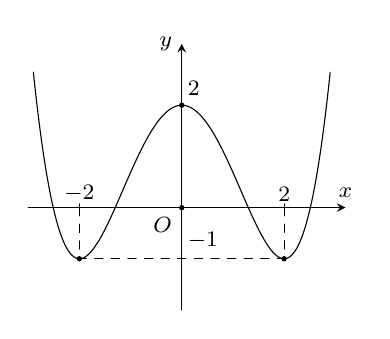
\begin{tikzpicture}[>=stealth,line join=round,line cap=round,font=\footnotesize,scale=0.65]
	\draw[->] (0,-2)--(0,3.2)node[left]{$y$};
	\foreach \y in {-1,2}
	\draw[shift={(0,\y)}] (2pt,0)--(-2pt,0) node[above right] {\footnotesize $\y$} ;
	\draw[->] (-3,0)--(3.2,0)node[above]{$x$};
	\foreach \x in {-2,2}
	\draw[shift={(\x,0)}] (0,2pt)--(0,-2pt) node[above] {\footnotesize $\x$};
	\fill (0,0) node[below left]{\footnotesize $O$} circle(1.5pt);
	\fill (0,2) circle(1.5pt) (-2,-1) circle(1.5pt) (2,-1)circle(1.5pt);
	\draw[samples=150,smooth,domain=-2.9:2.9] plot(\x,{3/16*(\x)^4-3/2*(\x)^2+2});
	\draw[dashed] (-2,0)--(-2,-1)--(2,-1)--(2,0);
	\end{tikzpicture}}
	\loigiai{
	Đặt $ g(x)=f(f(x)) $, suy ra
	\begin{align*}
	 g'(x)=f'(x)\cdot f'(f(x)) =0 \Leftrightarrow \hoac{&f'(x)=0\\&f'(f(x))=0}\Leftrightarrow \hoac{&x=0\\  &x=\pm 2\\& f(x)=0\\ &f(x)=\pm 2.}
	\end{align*}	
	Ta xét các trường hợp sau
	\begin{itemize}
		\item $ f(x)=0  $ có $ 4 $ nghiệm đôi một khác nhau $ a $, $ b $, $ c $ và $ d $.
		\item $ f(x)=2 $ có $ 3 $ nghiệm phân biệt $ x=0 $ và $ x=m $, $ x=n $.
		\item $ f(x)=-2 $ vô nghiệm.
		\end{itemize}
	Phương trình $ g'(x) =0$ có $ 8 $ nghiệm đơn đôi một khác nhau và  có $ 1 $ nghiệm $ x=0 $ bội $ 2 $.\\
	Vậy hàm số $ y=f(f(x)) $ có $ 8 $ điểm cực trị.
	}
\end{ex}
\begin{ex}%[GHK1, Nguyễn Khuyến-TPHCM, 2019]%[Nguyễn Anh Tuấn, 12EX1-20]%[2D1G5-2]
	Cho hàm số $ y=f(x) =x^3+3x^2+2$ và phương trình $ ||f(x)+m|+m|=n $ có $ 8 $ nghiệm phân biệt với $ m\in (-6;-2) $. Khẳng định nào sau đây đúng?
	\choice
	{$ \heva{& -6<m<-4 \\ & 2<n<-6-2m} $}
	{$ \heva{& -3<m<-2 \\ & 6+2m<n<2} $}
	{$ \heva{& -3<m<-2 \\ & -m<n} $}
	{\True $ \heva{& -3<m<-2 \\ & \hoac{& 0<n<6+2m \\ &2<n<-m}} $}
	\loigiai{
	Hàm số $ g(x)=f(x)+m=x^3+3x^2+2+m $ có bảng biến thiên như sau
	\begin{center}
		
\begin{tikzpicture}[>=stealth]
		\tkzTabInit[nocadre=false,lgt=2,espcl=2.5,deltacl=0.5]
		{$x$/.6 ,$g'(x)$/.6,$f(x)$/2,$ g(x) $/2}
		{$-\infty$ , $-2$ , $0$ , $+\infty$}
		\tkzTabLine{ , + , $0$ , - , $0$ , + , }
		\tkzTabVar{-/$-\infty$ , +/$6$ , -/$2$ , +/$+\infty$}
		\tkzTabVar{-/$-\infty$ , +/$6+m$ , -/$2+m$ , +/$+\infty$}
		\end{tikzpicture}
		\end{center}	
	Vì $ -6<m<-2 $ nên $ m+2<0 $, $ m+6>0 $.\\ Từ đó, phương trình $ g(x)=0 $ có $ 3 $ nghiệm phân biệt $ x_1 $, $ x_2 $, $ x_3 $ thỏa mãn $ x_1<-2<x_2<0<x_3 $.\\
	Do đó, hàm số $ y=|f(x)+m|+m $ có bảng biến thiên như sau
	\begin{center}
		
\begin{tikzpicture}[>=stealth]
		\tkzTabInit[nocadre=false,lgt=3,espcl=2,deltacl=0.5]
		{$x$/.6 ,$|g(x)|$/2,$ |g(x)|+m $/2}
		{$-\infty$ ,$ x_1 $, $-2$ ,$ x_2 $, $0$ ,$ x_3 $, $+\infty$}
		\tkzTabVar{+/$+\infty$ , -/$0  $,+/$6+m$ ,-/$ 0 $, +/$-2-m$ ,-/$ 0 $, +/$+\infty$}
		\tkzTabVar{+/$+\infty$ , -/$m  $,+/$6+2m$ ,-/$ m $, +/$-2$ ,-/$ m $, +/$+\infty$}
		\end{tikzpicture}
	\end{center}
	\begin{enumerate}[TH.1]
		\item Khi $ m=-3 $, tức là $ 6+2m=0 $.\\  Hàm số $ y=|f(x)+m|+m $ có bảng biến thiên như sau
		\begin{center}
			
\begin{tikzpicture}[>=stealth]
			\tkzTabInit[nocadre=false,lgt=2.2,espcl=2,deltacl=0.5]
			{$x$/.6 ,$|g(x)|+m$/2}
			{$-\infty$ ,$ x_1 $, $-2$ ,$ x_2 $, $0$ ,$ x_3 $, $+\infty$}
			\tkzTabVar{+/$+\infty$ , -/$-3  $,+/$0$ ,-/$ -3 $, +/$-2$ ,-/$ -3 $, +/$+\infty$}
			\end{tikzpicture}
		\end{center}
	Từ bảng biến thiên của hàm số $ y=|g(x)|+m $, suy ra phương trình $ ||g(x)|+m|=n $ có $ 8 $ nghiệm phân biệt khi và chỉ khi $ \heva{& m=-3 \\ & 2<n<3.}$
		\item Khi $ m>-3 $, tức là $ m>-3 $. Hay là $ -3<m<-2 $ và $ -m>6+2m $.\\ Phương trình $ |g(x)|+m=0 $ có $ 4 $ nghiệm phân biệt nên phương trình $ ||g(x)|+m|=n $ có $ 8 $ nghiệm phân biệt khi và chỉ khi $ \heva{& -3<m<-2 \\ & 2<n<-m} $ hoặc là $ \heva{& -3<m<-2 \\ & 0<n<6+2m.} $
		\item Khi $ -6<m<-4 $, tức là $ 6+2m<-2 $.\\ Phương trình $ ||g(x)|+m|=n $ có $ 8 $ nghiệm phân biệt khi và chỉ khi $ \heva{& -6<m<-4 \\ & 6+2m<n<-m.} $
		\item Khi $ m=-4 $.\\ Hàm số $ y=|f(x)+m|+m $ có bảng biến thiên như sau
		\begin{center}
			
\begin{tikzpicture}[>=stealth]
			\tkzTabInit[nocadre=false,lgt=2.2,espcl=2,deltacl=0.5]
			{$x$/.6 ,$|g(x)|+m$/2}
			{$-\infty$ ,$ x_1 $, $-2$ ,$ x_2 $, $0$ ,$ x_3 $, $+\infty$}
			\tkzTabVar{+/$+\infty$ , -/$-4 $,+/$-2$ ,-/$ -4 $, +/$-2$ ,-/$ -4 $, +/$+\infty$}
			\end{tikzpicture}
		\end{center}
		Phương trình $ ||g(x)|+m|=n $ có $ 8 $ nghiệm phân biệt khi và chỉ khi $ \heva{& m=-4 \\ & 2<n<4.}$
		\item Khi $ -4<m<-3 $, tức là $ -2<6+2m<0 $.\\ Phương trình $ ||g(x)|+m|=n $ có $ 8 $ nghiệm phân biệt khi và chỉ khi $ \heva{& -4<m<-3 \\ & 2<n<-m.}$
	\end{enumerate}}
\end{ex}
\begin{ex}%[GHK1, Nguyễn Khuyến-TPHCM, 2019]%[Nguyễn Anh Tuấn, 12EX1-20]%[2D1G3-5]
	Cho biểu thức $ P=\left(\dfrac{a^2}{b}-\dfrac{4b^2}{a}\right)(b-a)^2+8\sqrt{\left(7+5\sqrt{2}\right)(ab-a^2)\left[4\left(\sqrt{2}+1\right)b+a\right]} $ với $ a $, $ b $ là hai số thực thỏa mãn $ 0<a<-4\left(1+\sqrt{2}\right)b $. Giá trị lớn nhất của $ \left(5\sqrt{2}-7\right)P $ thuộc khoảng nào sau đây?
	\choice
	{$ (1;5) $}
	{$ (5;10) $}
	{\True $ (10;20) $}
	{$ (-5;5) $}
	\loigiai{
	Đặt $ m=\sqrt{2}+ 1$, suy ra $ 7+5\sqrt{2}=\left(\sqrt{2}+1\right)^3=m^3 $.\\
	Từ biểu thức $ P $ và điều kiện $ 0<a<-4mb $, suy ra $ b<0<a $.\\
	Áp dụng bất đẳng thức Bunhiacốpxki, có 
	$$ (a-2b)^2=\left(\sqrt{-b}\cdot \dfrac{a}{\sqrt{-b}}+\sqrt{a}\cdot \dfrac{-2b}{\sqrt{a}}\right)^2\leq (a-b)\left(\dfrac{a^2}{-b}+\dfrac{4b^2}{a}\right).$$	
	Vậy, ta có $ \dfrac{a^2}{-b}+\dfrac{4b^2}{a}\geq \dfrac{(a-2b)^2}{a-b} $. Từ đó, suy ra\\
	$$\left(\dfrac{a^2}{b}-\dfrac{4b^2}{a}\right)(b-a)^2\leq (b-a)(a-2b)^2.$$
	Lại có
	\begin{align*}
		m^3(ab-a^2)(4mb+a)&=m^3a(b-a)(4mb+a)\\
		&=m(a-b)[(1+2m)a(-4mb-a)]\leq m(a-b)[2ma-4mb^2]\\
		&=4m^3(a-b)(a-2b)^2.
	\end{align*}
	Suy ra $ 8\sqrt{m^3(ab-a^2)(4mb+a)}\leq 16\sqrt{m^3}\sqrt{(a-b)(a-2b)^2} $.\\
	Do đó, $ P\leq -t^2+16\sqrt{m^3}t\leq 16m^3 $ với $ t=\sqrt{(a-b)(a-2b)^2} $.\\
	Vậy $ \left(5\sqrt{2}-7\right)P\leq 16\left(5\sqrt{2}-7\right)(7+5\sqrt{2}) =16$.
	}
\end{ex}
\begin{ex}%[GHK1, Nguyễn Khuyến-TPHCM, 2019]%[Nguyễn Anh Tuấn, 12EX1-20]%[2D1G5-3]
	Cho hàm số $ y=f(x) $ và $ y=g(x) $ có đạo hàm trên $ \mathbb{R} $ và có bảng biến thiên như hình dưới đây
	\begin{center}
		
\begin{tikzpicture}[>=stealth]
		\tkzTabInit[nocadre=false,lgt=1.2,espcl=2.5,deltacl=0.5]
		{$x$/.6 ,$f(x)$/2,$ g(x)$ /2}
		{$-\infty$ ,$ x_1 $, $x_0$ ,$ x_2 $ , $+\infty$}
		\tkzTabVar{-/$-\infty$ , +/$ $,R,-/$ $, +/$+\infty$}
		\tkzTabVar{+/$+\infty$ , -/$ $,R,+/$ $, -/$-\infty$}
		\end{tikzpicture}
		\end{center}
	Biết rằng phương trình $ f(x)=g(x) $ có nghiệm $ x_0  \in (x_1;x_2)$. Số điểm cực trị của hàm số $ y=|f(x)-g(x)| $ là
	\choice
	{\True $ 5 $}
	{$ 3 $}
	{$ 4 $}
	{$ 2 $}
	\loigiai{
	Đặt $ h(x)=f(x)-g(x) $, với $ x\in \mathbb{R} $. Khi đó, $ h'(x)=f'(x)-g'(x) $.\\
	Bảng biến thiên của hàm số $ y=h(x) $ như sau
		\begin{center}
			
\begin{tikzpicture}[>=stealth]
			\tkzTabInit[nocadre=false,lgt=2,espcl=2.5,deltacl=0.5]
			{$x$/.6 ,$f'(x)$/0.7,$g'(x)$/0.7,$ h'(x) $/0.7, $ h(x) $/2}
			{$-\infty$ , $x_1$ , $x_2$ , $+\infty$}
			\tkzTabLine{ , + , $0$ , - , $0$ , + , }
			\tkzTabLine{ , - , $0$ , + , $0$ , - , }
			\tkzTabLine{ , + , $0$ , - , $0$ , + , }
			\tkzTabVar{-/$-\infty$ , +/$h(x_1)$ ,-/$h(x_2)$ , +/$+\infty$}
			\end{tikzpicture}
		\end{center}
	Vậy hàm số $ y=h(x)=f(x)-g(x) $ có hai điểm cực trị.\\
	 Mặt khác, phương trình $ f(x)-g(x)=0 $ có nghiệm $ x_0\in (x_1;x_2) $ nên $ h(x_0)=0 $. Dựa vào bảng biến thiên của hàm số $ y=h(x) $, ta thấy phương trình $ h(x)=0 $ có ba nghiệm phân biệt. Vậy hàm số $ y=|f(x)-g(x)| $ có $ 5 $ điểm cực trị.
	}
\end{ex}
\begin{ex}%[GHK1, Nguyễn Khuyến-TPHCM, 2019]%[Nguyễn Anh Tuấn, 12EX1-20]%[2H1G3-6]
	Cho tứ diện $ ABCD $ có $ AB=a $, $ BC=b $, $ AD=c $ với $ a $, $ b $, $ c $ không đổi, $ AB\perp BC $, $ AB\perp AD$. Gọi $ (P) $ là mặt phẳng vuông góc với $ AB $, góc $ \widehat{\left(CD,(P)\right)} =\alpha$ (thay đổi), hai đường thẳng $ (\Delta_1) $,$ (\Delta_2) $ vuông góc với nhau, cắt nhau tại $ D $ và quay quanh điểm $ D $, điểm $ M $ thuộc mặt phẳng $ \left(\Delta_1,\Delta_2\right) $ thỏa $ \mathrm{d}[M;(\Delta_1)] =\mathrm{d}^2[M;(\Delta_2)]-\dfrac{c^2}{4}$ và $ \mathrm{d}[M;(\Delta_2)]\leq AD $. Thể tích lớn nhất của khối tứ diện $ ABCM $ bằng
	\choice
	{$ \dfrac{abc}{24}\left(\sqrt{16+9c^2}\right) +14$}
	{$ \dfrac{abc}{3} $}
	{$ \dfrac{ab}{6}\left(\sqrt{b^2+c^2}+c\right) $}
	{\True $\dfrac{abc}{24}\left(\sqrt{16+9c^2}+4\right)  $}
	\loigiai{
	\begin{center}
		\begin{tikzpicture}[line join=round,line cap=round,line width=.6pt,font=\footnotesize,scale=1]
		\coordinate[label=below left:$B$] (B) at (0,0);
		\coordinate[label=above left:$A$] (A) at (2,1.5);
		\coordinate[label=below right:$C$] (C) at (4,0);
		\coordinate[label=above right:$C'$] (C1) at ($(C)-(B)+(A)$);
		\coordinate[label=above left:$D$] (D) at ($(A)+(80:4)$);
		\coordinate[label=above right:$H$] (H) at (6,7);
			\coordinate[label=below right:$M$] (M) at (8,6);
				\coordinate[label=below right:$K$] (K) at ($(D)-(H)+(M)$);
				\coordinate[label=above right:$E$] (E) at ($(M)+(270:5)$);
				\coordinate[label=below left:$D'$] (D1) at ($(D)+(270:4.8)$);
			\draw (D)--(H)--(M)--(K)--(D)--(M);
		\draw (B)--(C)--(C1)--(D)--cycle (D)--(C);
		\draw[dashed] (C)--(A)--(C1) (D)--(A)--(B) (M)--(E) (D)--(D1);
		\draw ($ (A)!5pt!(C1)$)--($(A)!2!($($(A)!5pt!(C1)$)!.5!($(A)!5pt!(D)$)$)$)--($(A)!5pt!(D)$);
		\fill (A)circle(2pt) (B)circle(2pt) (C)circle(2pt) (C1)circle(2pt) (D)circle(2pt) (H)circle(2pt) (M)circle(2pt) (K)circle(2pt) (D1)circle(2pt) (E)circle(2pt);
		\end{tikzpicture}
		
		\end{center}
	Lấy điểm $ C' $ sao cho $ ABCC' $ là hình chữ nhật; $ H $, $ K $, $ E $ lần lượt là hình chiếu của điểm $ M $ trên $ \Delta_1 $, $ \Delta_2 $, $ (ABC) $ và $ D' $ là hình chiếu của $ D $ trên $ (ABC) $. Khi đó
	\begin{itemize}
		\item $ (DAC')\equiv (P) $.
		\item $ D' $ thuộc đường thẳng $ AC' $.
		\item Thể tích khối chóp $ ABCM $ là $ V=\dfrac{1}{3}\dfrac{ab}{2}ME $.
	\end{itemize}
	Do đó, $ ME\leq MD+DD'\leq MD+c $, đẳng thức xảy ra khi và chỉ khi $ D'\equiv $, tức là $ DA\perp (ABC) $.\\
	Lại có $$ MD=\sqrt{MH^2+MK^2}=\sqrt{\left(MK^2-\dfrac{c^2}{4}\right)^2+MK^2}=\dfrac{\sqrt{16MK^4+8(2-c^2)MK^2+c^4}}{4} .$$
	Xét hàm số $ f(x)=16x^2+8(2-c^2)x+c^4 $ với $ 0\leq x=MK^2\leq c^2 $, có $$ \max\limits_{[0;c^2]} f(x)=\max\{f(0);f(c^2)\}=9c^4+16c^2.$$
	Vậy $ \max MD=\dfrac{c\sqrt{9c^2+16}}{4} $, tức là $ \max ME=\dfrac{c}{4}\left(4+\sqrt{9c^2+16}\right) $.\\
	Kết luận $ \max V_{ABCM}=\dfrac{abc}{24}\left(4+\sqrt{9c^2+16}\right)$.	
	}
\end{ex}
\begin{ex}%[GHK1, Nguyễn Khuyến-TPHCM, 2019]%[Nguyễn Anh Tuấn, 12EX1-20]%[2D1G3-1]
	Cho hàm số $ y=f(x) $ có đạo hàm trên $ \mathbb{R} $, bảng biến thiên của hàm số $ y=f(x) $ như hình vẽ và $ f''(x)<0, \forall x\in (0;+\infty) $. Biết $ a$, $x $ thay đổi trên đoạn $ [0;2] $ và giá trị nhỏ nhất của biểu thức $ S=\dfrac{\left[(f'(x))^2+1\right]\left[2f'(0)+(a-x)f'(a)+6\right]}{\left[f\left(2-\sqrt{4-x}\right)+f(x)\right]^2\left[f\left(2-\sqrt{4-x}\right)+f(a)\right]} $ bằng $ \dfrac{m}{n} $ (phân số tối giản). Tổng $ m+n $ thuộc khoảng nào sau đây?
	\begin{center}
		
\begin{tikzpicture}[>=stealth]
		\tkzTabInit[nocadre=false,lgt=1.2,espcl=2.5,deltacl=0.5]
		{$x$/.6 ,$f(x)$/2}
		{$-\infty$ ,$ -3 $, $0$ ,$ 2 $ , $+\infty$}
		\tkzTabVar{+/$ $ ,-/$ $,R,+/$ 4$, -/$ $}
		\tkzTabIma{2}{4}{3}{$2$}
		\end{tikzpicture}
		\end{center}
	\choice
	{$ (20;25) $}
	{$ (95;145) $}
	{\True $ (45;75) $}
	{$ (75;95) $}
	\loigiai{
	Xét $ x\in [0;2] $, suy ra $ 2-\sqrt{4-2x} \in [0;2] $. Mặt khác, $ f''(x)<0, \forall x\in [0;2] $.\\
	Từ bảng biến thiên của hàm số $ y=f(x) $, suy ra
	$$f\left(2-\sqrt{4-2x}\right)\leq f(2);\quad f'(x)\geq f'(2);\quad f(x)\leq f(2).$$
	Lại có $ 2f'(0)+(a-x)f'(a)+6\geq 2f'(0)+(a-2)f'(a)+6 $, với $ x\in [0;2] $.\\
	Khi đó
	$$S\geq \dfrac{2f'(0)+(a-x)f'(a)+6}{64[4+f(a)]}\geq \dfrac{1}{64} \dfrac{2f'(0)+(a-2)f'(a)+6}{4+f(a)}.$$
	Ta chứng minh
	$$\dfrac{2f'(0)+(a-2)f'(a)+6}{4+f(a)}\geq 1.$$
	Thật vây, $ \dfrac{2f'(0)+(a-2)f'(a)+6}{4+f(a)}\geq 1 \Leftrightarrow f(a)+(2-a)f'(a)-2f'(0)-2\leq 0 $.\\
	Xét hàm số $ g(a)=f(a)+(2-a)f'(a)-2f'(0)-2 $ với $ a\in [0;2] $.\\ Khi đó
	$ g'(a)=(2-a)f''(a)\leq 0, \forall a\in[0;2] $. Do đó, $ g(a)\leq g(0)=0 $.\\ Điều này chứng tỏ, $\dfrac{2f'(0)+(a-2)f'(a)+6}{4+f(a)}\geq 1$ hay là $ S\geq \dfrac{1}{64} $.\\
	Dấu $ = $ xảy ra khi và chỉ khi $ x=2 $, $ a=0 $. Từ đó, $ m=1 $, $ n=64 $ nên $ m+n=65 $.
	}
\end{ex}
\Closesolutionfile{ans}
\begin{indapan}{10}
	{ans/ans-2-GHK1-4-NguyenKhuyen-TPHCM-20}
\end{indapan}